% \documentclass[tikz,convert={outfile=\jobname.svg}]{standalone}
\documentclass[tikz,convert=pdf2svg]{standalone}
%\usetikzlibrary{...}% tikz package already loaded by 'tikz' option
\usetikzlibrary{arrows, arrows.meta}
% \tikzset{
%   >=stealth',
% }
\usepackage{amsmath,amssymb}
\usepackage{ndtheme}

\begin{document}
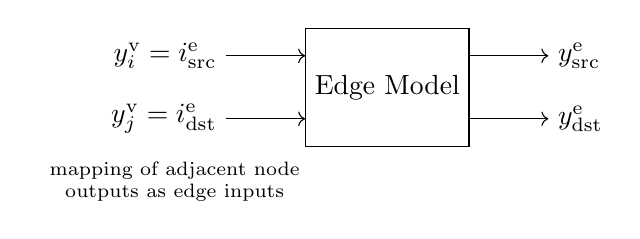
\begin{tikzpicture}[\ndtheme]
  \node[draw, minimum height=1.5cm](n){
    Edge Model
  };
  \draw[->](n.east)++(0,0.4)--++(1.0,0) node[right]{$y^{\mathrm e}_{\mathrm{src}}$}; \draw[->](n.east)++(0,-0.4)--++(1.0,0) node[right]{$y^{\mathrm e}_{\mathrm{dst}}$};

  \draw[<-](n.west)++(0,0.4)--++(-1.0,0) node[left]{$y^{\mathrm v}_{i}=i^{\mathrm e}_{\mathrm{src}}$};
  \draw[<-](n.west)++(0,-0.4)--++(-1.0,0) node[left]{$y^{\mathrm v}_{j}=i^{\mathrm e}_{\mathrm{dst}}$};

  \node[text width=3.5cm, align=center, font=\scriptsize] at ([xshift=-2.7cm, yshift=-1.2cm]n) {mapping of adjacent node outputs as edge inputs};
\end{tikzpicture}
\end{document}
